\documentclass[a4paper]{report}
\usepackage{graphicx,caption}
\usepackage[utf8]{inputenc}

\title{Metodologias para a construção de ontologias} 
\author{}
\date{} % para este exemplo, deixarei a data vazia

\begin{document}
\pagestyle{plain}
\maketitle

\subsection{Método Cyc}

\qquad \textit{CyC} é um projeto do \textit{Microelectronics and Technology Computer Corporation (MCC) em Austin, Texas}, que fornece uma base para o raciocínio de senso comum através do desenvolvimento de ontologias para uma ampla variedade de aplicações específicas de domínio. Todo o conhecimento em CyC é representado de forma declarativa na forma de afirmações em uma variante da lógica de primeira ordem chamado CYCL. A própria base de conhecimento CYC contém afirmações simples, motor de inferência pode ser usado para derivar novas afirmações que utilizam esta base de conhecimento.
As ontologias subjacentes CYC são organizados em conjuntos de módulos conhecidos como microteorias. Cada microteoria captura o conhecimento e o raciocínio necessário para algumas de domínio particular, como espaço, tempo, causalidade, ou agentes.

Podem existir múltiplos microteorias para um determinado domínio, refletindo as diferentes perspectivas e suposições feitas para pessoas modelar esse domínio. Neste sentido, CYC não é uma ontologia integrado monolítica, ao contrário, é uma rede de microteorias para um conjunto de domínios cuja união abrange os diferentes compromissos da ontologia que podem ser feitas dentro desses domínios %\cite{Andreia2010}.
	A Figura 1 ilustra os três processos que foram conduzidos no desenvolvimento da
base de conhecimento Cyc em 1990 por Douglas Lenat e Ramanathan Guha (apud LENAT e GUHA, 1990 111 FERNANDEZ, GOMEZ-PEREZ e CORCHO, 2004).

\begin{figure}[h] 
\centering % para centralizarmos a figura
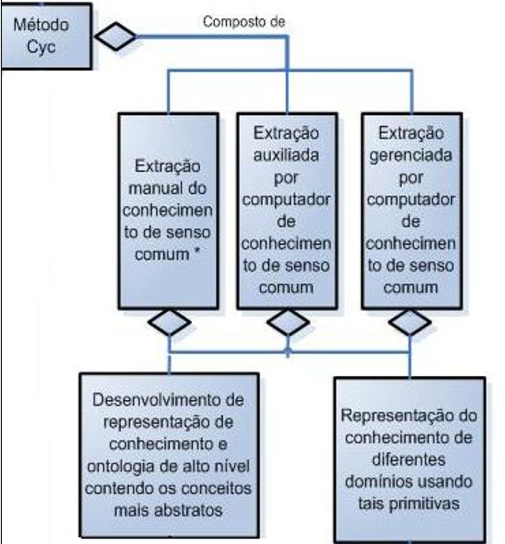
\includegraphics[scale=0.6]{Figuras/1.png} % leia abaixo
\caption[Processos e atividades propostas pelo método Cyc]{Processos e atividades propostas pelo método Cyc. %Fonte: \cite{DanielaLucas2008}
}
\end{figure}

\pagebreak

Tabela 01 – Tabela abreviada do método Cyc
                                  
\begin{figure}[h] 
\centering % para centralizarmos a figura
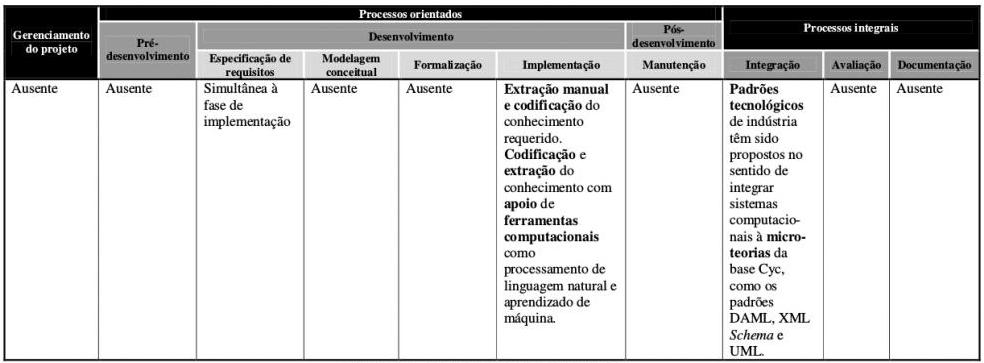
\includegraphics[scale=0.3]{Figuras/2.png} % leia abaixo
\caption{Fonte %: \cite{DanielaLucas2008}
}
\end{figure}

\subsection{Metodologia de Gruninger e Fox}    

\qquad Esta metodologia baseia-se na experiência em desenvolvimento de ontologia do projeto Tove dentro do domínio de processos e atividades de negócios de
modelagem. Essencialmente, ele envolve a construção de um modelo lógico de o conhecimento que está a ser especificado por meio da ontologia. Este modelo não é construído diretamente. Primeiro, uma descrição informal é feita das especificações para
serem atendidas pela ontologia e, em seguida, esta descrição é formalizada. As medidas propostas são as seguintes:\newline
1. A captação de cenários motivadores;\newline
2. Formulação de perguntas informais de competência;\newline
3. Especificação da terminologia da ontologia dentro de uma linguagem formal:\newline
3.1. Obtendo terminologia informal;\newline
3.2. Especificação da terminologia formal;\newline
4. Formulação de questões formais de competência usando a terminologia da ontologia.\newline
5. Especificação de axiomas e definições para os termos na ontologia dentro da linguagem formal.\newline
6. Estabelecer condições para a caracterização da integralidade da ontologia.\newline
6.1. Ontologias desenvolvida utilizando esta metodologia.\newline
6.2. Aplicações utilizando ontologias desenvolvida com esta metodologia. \newline
6.3. Empresa Projeto Workbench.\newline
6.4. Abastecimento Integrado Cadeia Project Management agentes.\newline
6.5. análise da metodologia.%\cite{VariosAutores2009}

\pagebreak

A Figura a seguir ilustra tal metodologia:

\begin{figure}[h] 
\centering % para centralizarmos a figura
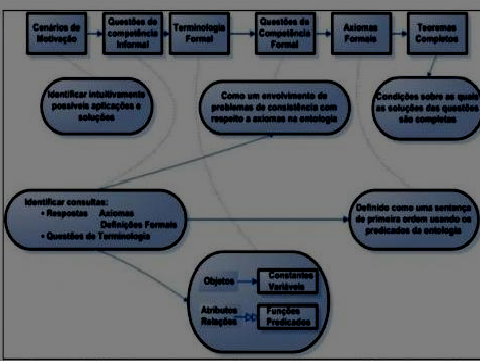
\includegraphics[scale=0.65]{Figuras/3.png} % leia abaixo
\caption[Procedimentos propostos na metodologia de Gruninger e Fox]{Procedimentos propostos na metodologia de Gruninger e Fox. %Fonte: \cite{DanielaLucas2008}
}
\end{figure}

Tabela 2 – Tabela abreviada da metodologia de Gruninger e Fox

\begin{figure}[h] 
\centering % para centralizarmos a figura
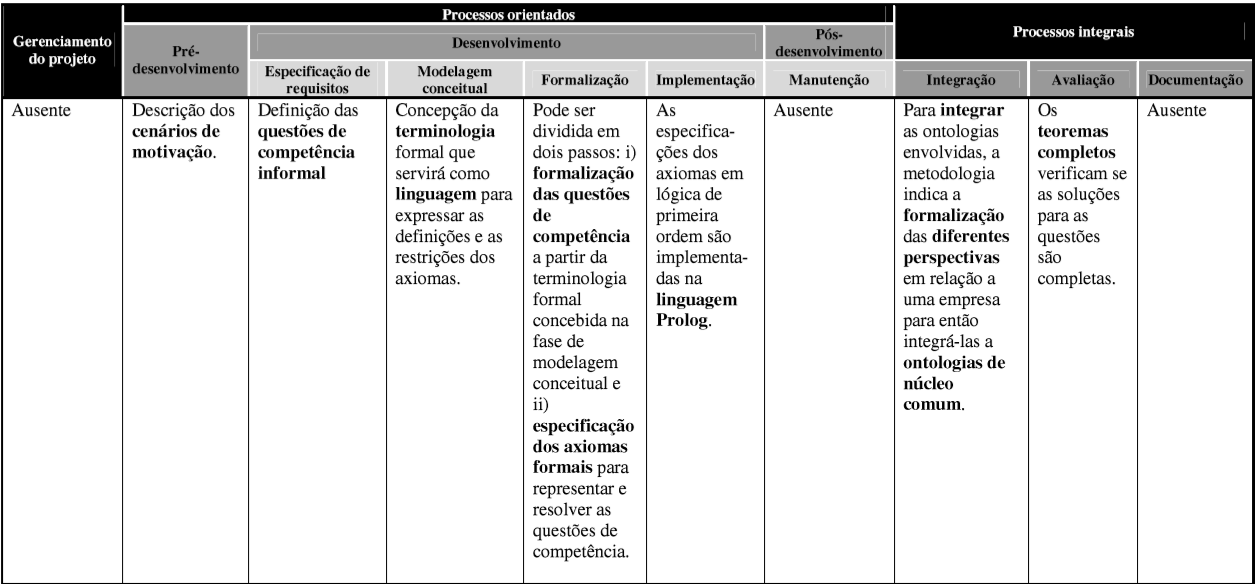
\includegraphics[scale=0.3]{Figuras/4.png} % leia abaixo
\caption{Fonte%: \cite{DanielaLucas2008}
}
\end{figure}

\subsection{Método de Uschold e King} 
\qquad Uschold apresenta uma metodologia unificada, combinando as "melhores" partes de OE e Tove em um unificado método (apud Uschold, 1996). O primeiro passo é definir a finalidade da ontologia, ou seja, porque é a ontologia sendo construída. Isto pode ser feito de várias maneiras, por exemplo para identificar os utilizadores destinados, ou como no projeto com Tove, cenários de motivação e perguntas de competência, ou um documento de requisitos do usuário. Em seguida, o desenvolvedor deve decidir o nível de formalidade que a ontologia tem que ter. Na próxima fase, o desenvolvedor precisa encontrar os conceitos que deveriam estar na ontologia e as relações entre eles. Uschold prefere ir pelo means-out maneira ao definir termos e relacionamentos. Quando se trata de construir a ontologia o autor descreve quatro diferentes abordagens. O primeiro deles é pular as etapas anteriores e usar um editor de ontologias para definir os termos e axiomas %\cite{SeveralAuthorUFF2011}. 

Em segundo lugar, fazer os passos anteriores e, em seguida, iniciar uma codificação formal. A terceira abordagem é produzir um documento intermediário que consiste em os termos e definições que apareceram na etapa anterior, este documento pode ser o resultado final, ou seja especificação do código formal ou documentação para ele ser. O quarto e aproximação final é identificar os termos formais a partir do conjunto de termos informais. A parte final presente no Uschold é o ciclo de avaliação ou a revisão, onde a ontologia desenvolvida é comparada com as questões da competência ou as necessidades dos utilizadores %\cite{SeveralAuthor2011}. 

A Figura 05 apresenta tais estágios envolvidos na construção de uma ontologia:

\begin{figure}[h] 
\centering % para centralizarmos a figura
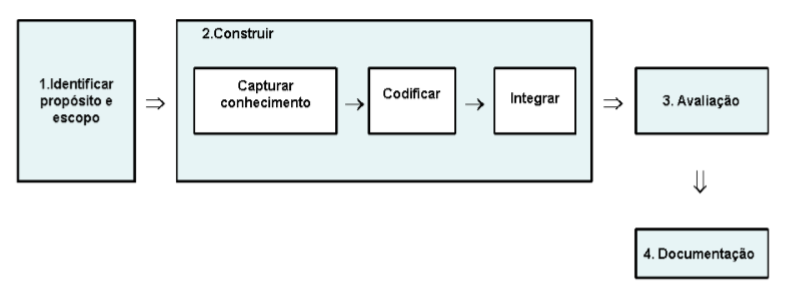
\includegraphics[scale=0.5]{Figuras/5.png} % leia abaixo
\caption{Estágios do método de Uschold e King.
Fonte: Adaptado de Uschold e King (1995)}
\caption[Estágios do método de Uschold e King]{Estágios do método de Uschold e King. %Fonte: \cite{DanielaLucas2008}
}
\end{figure}

\pagebreak
Tabela 03 - Tabela abreviada do método de Uschold e King

\begin{figure}[h] 
\centering % para centralizarmos a figura
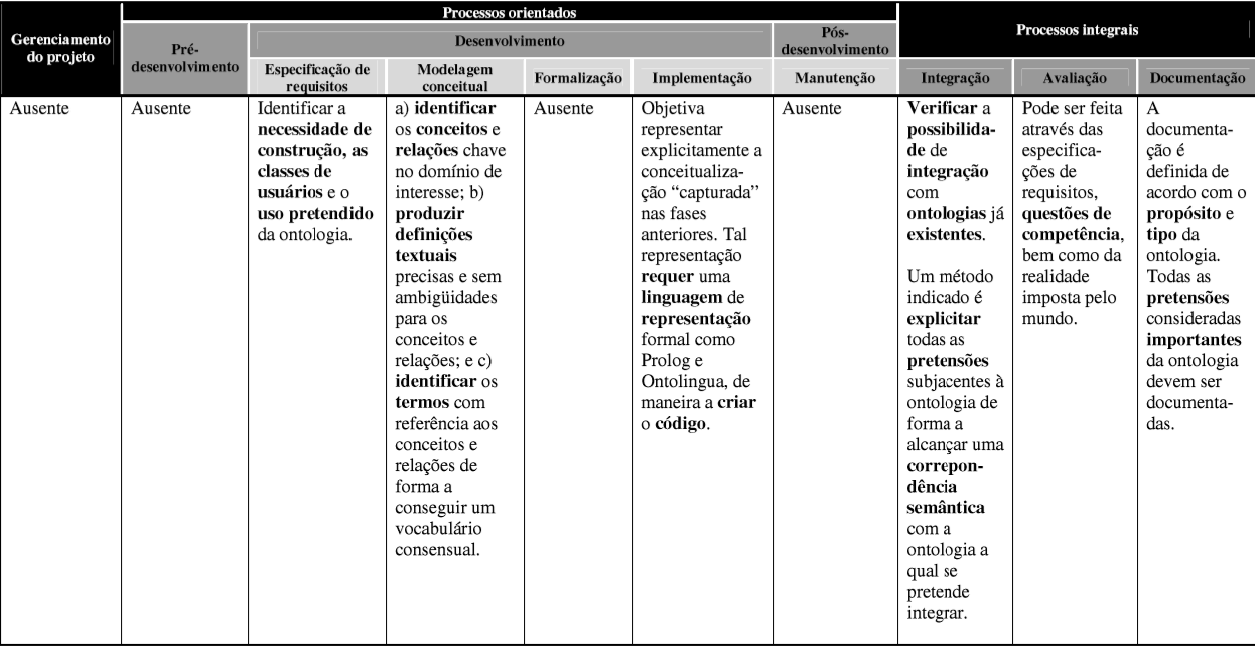
\includegraphics[scale=0.3]{Figuras/6.png} % leia abaixo
\caption{Fonte%: \cite{DanielaLucas2008}
}
\end{figure}

\subsection{Método Kactus} 
\qquad Kactus é um método amplamente utilizado para o desenvolvimento de sistemas baseados em conhecimento, em que ontologias desempenham um papel importante. O projeto Kactus foi um projecto de acompanhamento que centrou-se na questão do desenvolvimento da ontologia. Uma abordagem de engenharia é adotada, salientando design modular, redesenhar e reutilizar. Uma ontologia é construída a partir de uma biblioteca de ontologias de pequena escala, que requer mapeamento entre as várias ontologias incluídas na desenvolvimento da nova ontologia. Dois tipos de funções de mapeamento são definidas entre o vocabulários de ontologias:
(I) não há nenhuma mudança na semântica de expressões da ontologia mapeada.
(II) uma alteração ocorre na semântica da ontologia mapeada como uma interpretação do que ocorre.

A seleção de ontologias relevantes a partir de uma biblioteca é suportado por um esquema de indexação para ontologias. Este caracteriza o contexto interpretação da utilização de uma ontologia segundo três dimensões: tipo de tarefa; método de resolução de problemas, e do tipo de domínio. O modular princípio de desenvolvimento é comum em engenharia ontológica e decorre do foco na reutilização. Embora o trabalho em funções de mapeamento está atualmente bastante limitado, a abordagem parece ter potencial em alfaiataria, ontologias para aplicação particular %\cite{VariosAutores2009}. 

\pagebreak

Tabela 04 – Tabela abreviada do método Kactus

\begin{figure}[h] 
\centering % para centralizarmos a figura
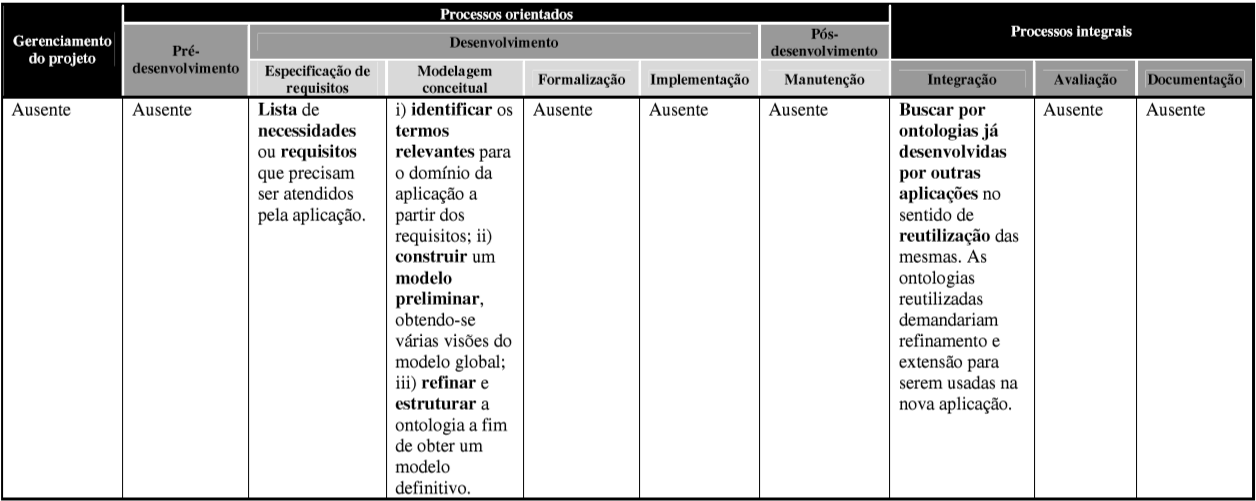
\includegraphics[scale=0.4]{Figuras/7.png} % leia abaixo
\caption{Fonte: \cite{DanielaLucas2008}}
\end{figure}

\subsection{Metodologia Methontology} 
\qquad A metodologia METHONTOLOGY é utilizada para construir ontologias a partir do zero (apud Fernández et al., 1997). O primeiro passo é especificar a finalidade da ontologia, o nível de formalidade e do escopo da ontologia. Em seguida, todo o conhecimento precisa ser coletado. Existem várias maneiras de fazer isso: através de brainstorming, entrevistas estruturadas e não estruturadas, análise formal e informal de textos e ferramentas de aquisição de conhecimento. Na fase de conceituação Fernández  primeiro propos a construção de um glossário de termos de todo o conhecimento possivelmente útil no domínio determinado. Em seguida, os termos são agrupados de acordo com conceitos e verbos, e estes são reunidos para formar tabelas de fórmulas e regras. A próxima coisa a fazer é verificar se existem quaisquer ontologias já existentes que podem e devem ser usados. O resultado da fase de implementação é a ontologia codificada em uma linguagem formal, que pode ser avaliada (verificados e validados) de acordo com algumas referências. A parte final consiste na documentação \cite{VariosAutores2009}. 
 
Cada fase resulta em um documento que descreve a ontologia desenvolvida até agora. Durante o ciclo de vida temos a atividade de suporte. E nela se engloba a aquisição do conhecimento, documentação e avaliação conforme pode ser visto na figura a seguir:

\begin{figure}[h] 
\centering % para centralizarmos a figura
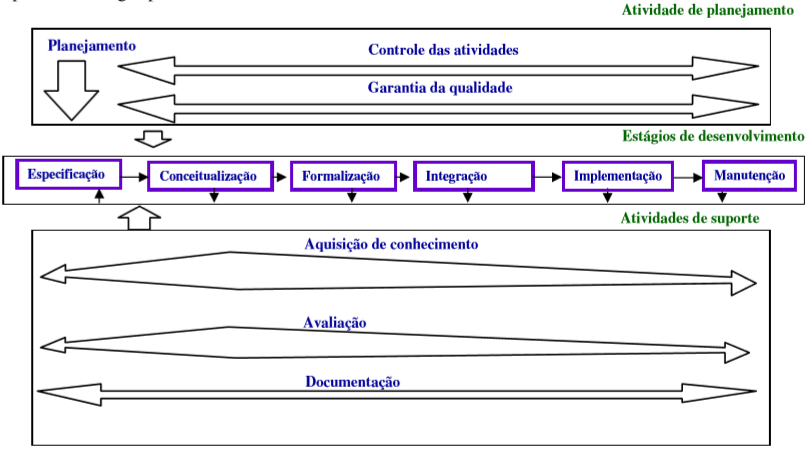
\includegraphics[scale=0.5]{Figuras/8.png} % leia abaixo
\caption[Estágios e atividades do ciclo de vida da ontologia]{Estágios e atividades do ciclo de vida da ontologia. Fonte: \cite{DanielaLucas2008}}
\end{figure}

\pagebreak
Tabela 05 – Tabela abreviada da metodologia Methontology

\begin{figure}[h] 
\centering % para centralizarmos a figura
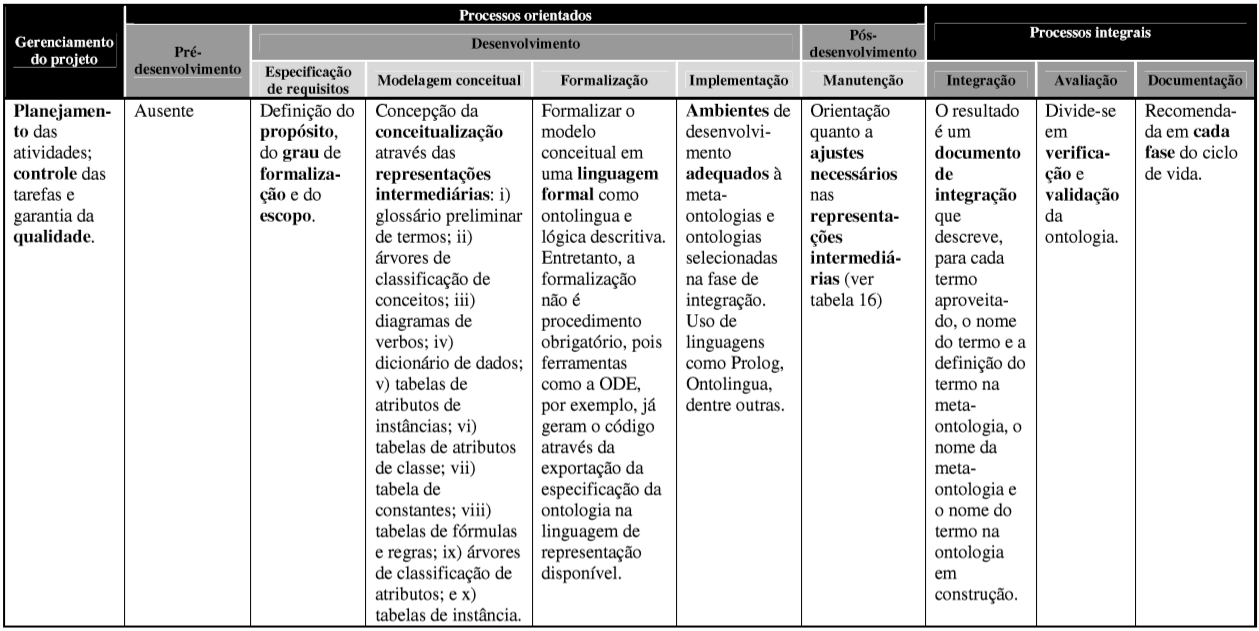
\includegraphics[scale=0.4]{Figuras/9.png} % leia abaixo
\caption{Fonte: \cite{DanielaLucas2008}}
\end{figure}

\subsection{Método Sensus} 
\qquad O método baseado na Sensus é uma abordagem top-down para derivar ontologias específicas de domínio de grandes ontologias. As etapas são as seguintes:\newline 
1) Uma série de termos são tomados como semente;\newline
2) Esses termos de sementes estão ligados à mão para SENSUS;\newline
3) Todos os conceitos no caminho dos termos de sementes para a raiz SENSUS estão incluídos;\newline
4) Termos que poderiam ser relevantes no domínio e não têm ainda aparecido são adicionados;\newline 
5) Finalmente, para os nós que têm um grande número de caminhos através deles,
toda a subárvore sob o nó é adicionado às vezes, baseada na idéia de que, se muitos dos gânglios em uma sub-árvore, foram encontrados para ser relevante, em seguida, os outros nós na sub-árvore é provável que sejam relevantes. Esta metodologia utiliza a ontologia existente, onde a fusão será complexa devido a diferentes estruturas \cite{SeveralAuthorUFF2011}.

Tabela 06 – Tabela abreviada do método Sensus

\begin{figure}[h] 
\centering % para centralizarmos a figura
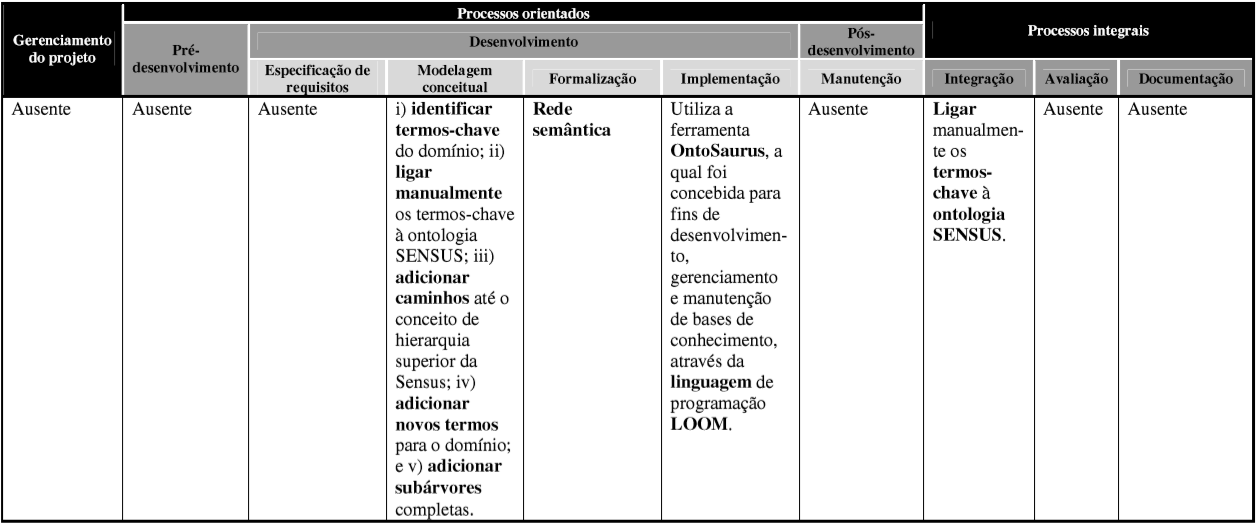
\includegraphics[scale=0.4]{Figuras/10.png} % leia abaixo
\caption{Fonte: \cite{DanielaLucas2008}}
\end{figure}

\subsection{Método 101} 
\qquad O método 101 foi criado por  Natalya F. Noy e Deborah L. McGuinness com base em experiências no desenvolvimento das ontologias de alimentos e vinhos, utilizando para isso o conceituadissimo software para a criação e edição de ontologias o Protégé-2000. Noy e McGuinness (2001, p.2) disseram em sua obra que não existe uma única maneira mais adequada para a construção de ontologias, e portanto não definiriam a melhor ontologia. A idéia desse método surgiu quando as autoras tiveram a idéia de compartilhar  as suas experiências para a construção de ontologias, de modo a ser útil em algum momento para outras pessoas, em outros projetos. A origem do método segundo as autoras foram baseadas na literatura do POO (paradigmas orientados a objetos), contudo para o desenvolvimento de ontologias cada um deles, é claro, tem as suas particularidades, diferindo em alguns aspectos. \cite{VariosAutores2009} Para a execução do método 101, sete passos são considerados fundamentais no processo de construção da ontologia, conforme mostrado na figura 11.

\pagebreak

\begin{figure}[h] 
\centering % para centralizarmos a figura
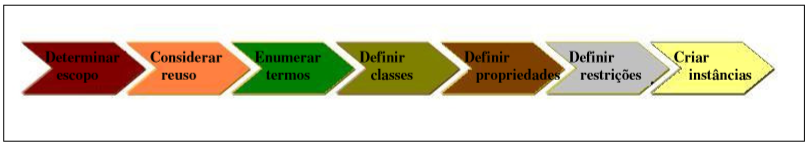
\includegraphics[scale=0.6]{Figuras/11.png} % leia abaixo
\caption[Processo de desenvolvimento de ontologias.]{Processo de desenvolvimento de ontologias.. Fonte: \cite{DanielaLucas2008}}

\end{figure}

Tabela 07 – Tabela abreviada do método 101

\begin{figure}[h] 
\centering % para centralizarmos a figura
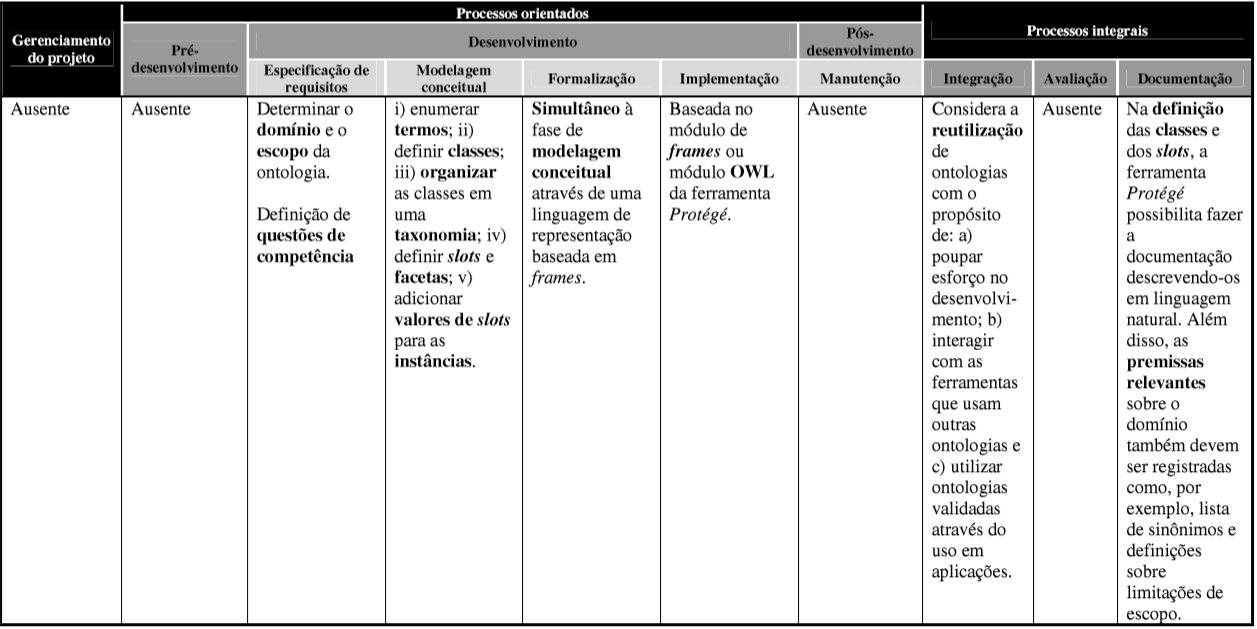
\includegraphics[scale=0.4]{Figuras/12.png} % leia abaixo
\caption{Fonte: \cite{DanielaLucas2008}}
\end{figure}

\subsection{Metodologia e Norma para construção de vocabulários controlados} 
\qquad O objetivo de vocabulários controlados é organizar as informações e
para fornecer terminologia para catalogar e recuperar informações. Enquanto
capturando a riqueza de termos de variantes, vocabulários controlados também
promovem a coerência em termos preferenciais e da atribuição dos mesmos termos de conteúdo semelhante.
	
	Dado que uma meta compartilhada da comunidade património cultural,
é melhorar o acesso às artes visuais e informações de cultura material,
vocabulários controlados são essenciais. Eles são necessários para a indexação
fase porque sem eles catalogadores não vão usar consistentemente o mesmo
termo para se referir à mesma pessoa, lugar ou coisa. No processo de recuperação,
vários usuários finais podem usar diferentes sinônimos ou mais termos genéricos para
referem-se a um dado conceito. Os usuários finais muitas vezes não são especialistas e, portanto, precisam para serem guiados porque eles podem não saber o termo correto.
	As funções mais importantes de um vocabulário controlado são para reunir termos e sinônimos variantes para os conceitos e associar conceitos em uma ordem lógica ou classificá-los em categorias. Por exemplo: são um indicador de rosa e Catherine roda são a mesma coisa? Como está relacionado vidro pote metal para o vidro mais geral termo marcado? As ligações e relações em um vocabulário controlado podem garantir que estas conexões são definidas e mantidas, tanto para catalogação quanto para recuperação \cite{VariosAutores2009}.\linebreak

Tabela 08 – Tabela abreviada da norma ANSI/NISO Z39.19-2005

\begin{figure}[h] 
\centering % para centralizarmos a figura
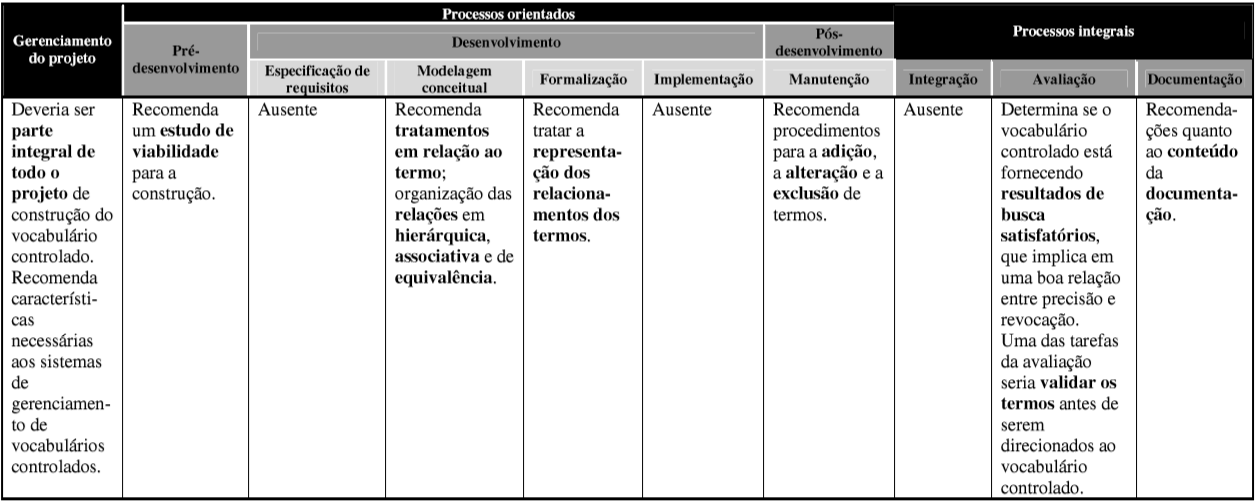
\includegraphics[scale=0.4]{Figuras/13.png} % leia abaixo
\caption{Fonte: \cite{DanielaLucas2008}}
\end{figure}

Tabela 09 – Tabela abreviada da metodologia proposta no manual da BITI

\begin{figure}[h]
\centering % para centralizarmos a figura
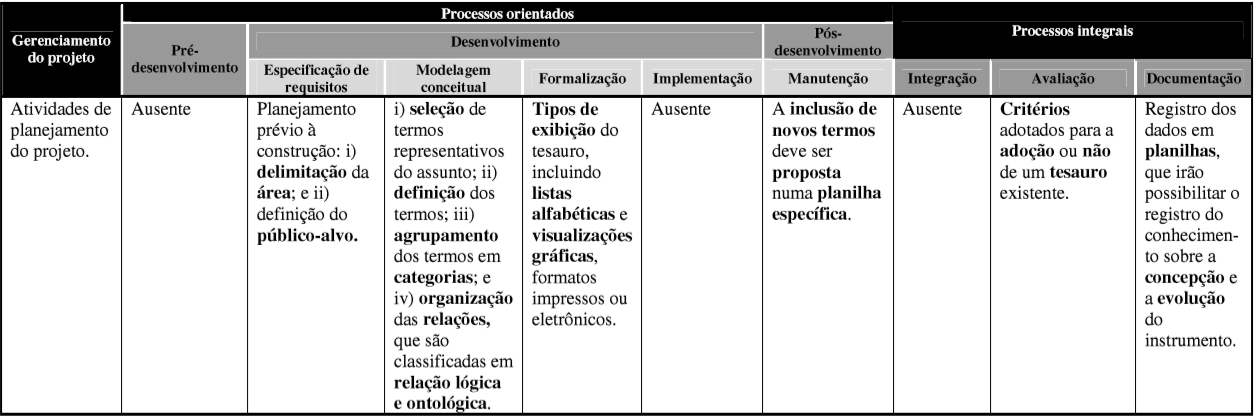
\includegraphics[scale=0.4]{Figuras/14.png} % leia abaixo
\caption{Fonte: \cite{DanielaLucas2008}}
\end{figure}

\end{document}